
\section{Auswertung}
\subsection{Bestimmung der Zeitkonstante über Auf- und Entladungsvorgang}
Zur Bestimmung der Zeitkonstante $RC$ werden die Messdaten wie in Tabelle(\ref{tab:1})
in ein Diagramm (\ref{fig:6}) dargestellt und mit Hilfe einer linearen Ausgleichsrechnung
berechnet.
\begin{table}[H]
  \centering
  \caption{Tabelle zur Bestimmung der Zeitkonstante mit $U_\text{0}$ = $10V$}
    \begin{tabular}{c c c }
      \toprule \\
      $U_\text{c} / V$& $ln(\frac{U_\text{c}}{U_\text{0}})$ & $t /\si{\milli\second}$ \\
      \midrule \\
      10,0& -0,000 & 0,00 \\
      9,04& -0,100 & 0,10 \\
      8,48& -0,165 & 0,16 \\
      7,84& -0,243 & 0,24 \\
      7,12& -0,340 & 0,34 \\
      6,80& -0,386 & 0,40 \\
      6,16& -0,485 & 0,50 \\
      5,36& -0,624 & 0,66 \\
      4,88& -0,717 & 0,78 \\
      4,32& -0,839 & 0,96 \\
      3,76& -0,978 & 1,14 \\
      3,52& -1,044 & 1,24 \\
      3,28& -1,115 & 1,36 \\
      3,04& -1,191 & 1,50 \\
      2,72& -1,302 & 1,80 \\
      2,48& -1,394 & 2,06 \\
      2,32& -1,461 & 2,28 \\
      2,24& -1,496 & 2,50 \\
      2,16& -1,532 & 2,76 \\
      2,08& -1,570 & 3,00 \\
      2,08& -1,570 & 3,22 \\
      2,00& -1,609 & 3,38 \\
      2,00& -1,609 & 3,56 \\
      2,00& -1,609 & 3,86 \\
      2,00& -1,609 & 4,06 \\
      2,00& -1,609 & 4,30 \\
      2,00& -1,609 & 4,46 \\
      2,00& -1,609 & 4,48 \\
      2,00& -1,609 & 4,52 \\
      \bottomrule
    \end{tabular}
    \label{tab:1}
  \end{table}

\begin{figure}[H]
  \centering
  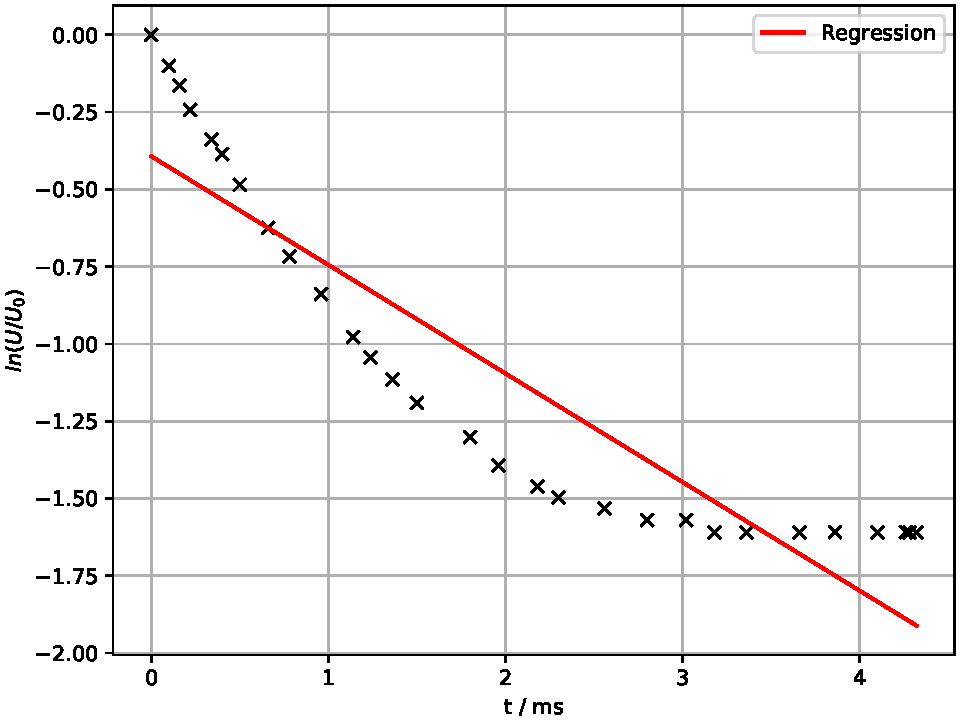
\includegraphics[width=\textwidth]{Diagramm1.pdf}
  \caption{Diagrammdarstellung vom Entladungsvorgang}
  \label{fig:6}
\end{figure}
\begin{figure}[H]
  \centering
  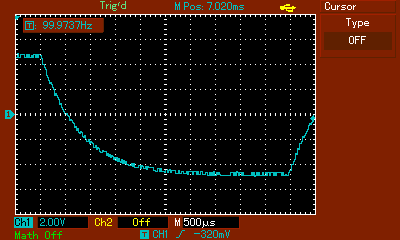
\includegraphics[width=\textwidth]{Entlade.jpg}
  \caption{Thermodruck vom Entladungsvorgang}
\end{figure}
Die Ausgleichsrechnungs allgemein lautet:
\begin{align}
  y & = m \cdot x + b \label{eq:9}\\
  m & = \frac {\bar{xy} - \bar{x} \cdot \bar{y}} {\bar{x^2} -\bar{x}^2}&  \label{eq:10}\\
  b & = \frac {\bar{y} \cdot \bar{x}^2 - \bar{xy} \cdot \bar{x}} {\bar{x^2}-\bar{x}^2}& \label{eq:11}
\end{align}
Für diese Ausgleichsrechnung wird die Formel (\ref{eq:1}) umgeschrieben und die erechnetet Werte lauten: \\
\newline
\centerline{$ln(\frac{U_\text{c}}{U_\text{0}}) = -\frac{1}{m} + b$}\\
\newline
\centerline{mit $m = (2,845 \pm 0,245) \cdot 10^{-3} \si{\second}$}\\
\newline
\centerline{und $b = (-0,393 \pm 0,074)$}
\newline
Dabei ist $m$ die Zeitkonstante $RC$.
\subsection{Bestimmung der Zeitkonstante über den Tiefpassvorgang}
Dabei wird die normierte Amplitude in Abhängigkeit von der Frequenz wie in der Tabelle(\ref{tab:2}) in
einen Diagramm dargestellt.
\begin{table}[H]
  \centering
  \caption{Tabelle von der Amplitude in Abhängigkeit der Frequenz mit $U_0 = 10V$}
    \begin{tabular}{c c}
      \toprule \\
      $\frac{A(\omega)}{U_\text{0}}$ & $\omega \,\, \text{in} \,\, Hz$ \\
      \midrule \\
      0.448 & 10\\
      0.448 & 20\\
      0.448 & 30\\
      0.440 & 40\\
      0.440 & 50\\
      0.432 & 60\\
      0.424 & 70\\
      0.416 & 80\\
      0.416 & 90\\
      0.400 & 100\\
      0.328 & 200\\
      0.264 & 300\\
      0.216 & 400\\
      0.176 & 500\\
      0.152 & 600\\
      0.135 & 700\\
      0.120 & 800\\
      0.112 & 900\\
      0.096 & 1000\\
      0.0448& 2000\\
      0.0296& 3000\\
      0.0224& 4000\\
      0.0180& 5000\\
      0.0152& 6000\\
      0.0128& 7000\\
      0.0112& 8000\\
      0.0100& 9000\\
      0.0090& 10000\\
      \bottomrule
    \end{tabular}
    \label{tab:2}
  \end{table}

\begin{figure}[H]
  \centering
  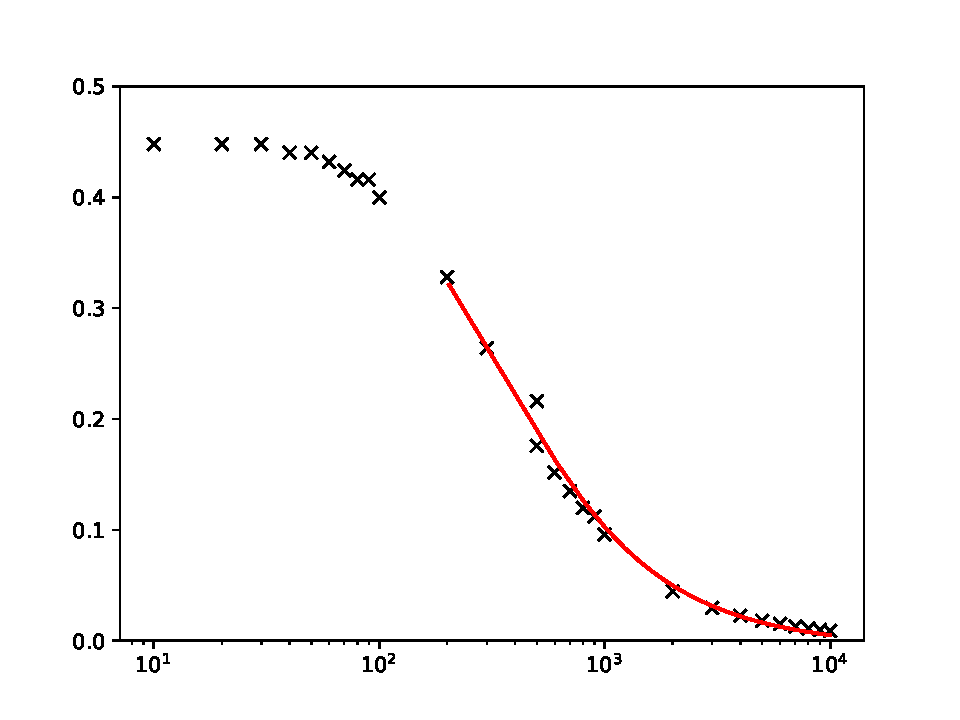
\includegraphics[width=\textwidth]{Diagramm2.pdf}
  \caption{Diagrammdarstellung von der relatvien Amplitude in Abhängigkeit der Frequenz}
  \label{fig:7}
\end{figure}
Für die nicht-lineare Ausgleichsrechnung wird die Gleichung (\ref{eq:7}) verwendet.
\begin{equation*}
  \frac{A}{U_0} = \frac{1}{\sqrt{1 + (\omega m)^2}}
\end{equation*}
\centerline{mit $m = (4,46 \pm \, 0.07) \cdot 10^{-3} \si{\second}$}
Wie vorhin ist $m$ die Zeitkonstante $RC$
\subsection{Bestimmung der Zeitkonstante mit Hilfe der Phasenverschiebung}
Es werden die Daten von der Tabelle(\ref{tab:3}) in einen Diagramm dargestellt und mit Hilfe
einer nicht-linearen Ausgleichsrechnung die Zeitkonstante bestimmt.
\begin{table}[H]
  \centering
  \caption{Tabelle zur Bestimmung der Zeitkonstante mit $\phi$ = $\frac{a}{b} \cdot 2\pi$}
    \begin{tabular}{c c}
      \toprule
      $\phi / \text{rad}$ & $\omega / \text{Hz}$  \\
      \midrule
       0.0000 &    10 \\
       0.0524 &    20 \\
       0.1070 &    30 \\
       0.2010 &    40 \\
       0.2821 &    50 \\
       0.3662 &    60 \\
       0.4057 &    70 \\
       0.4263 &    80 \\
       0.4755 &    90 \\
       0.4547 &    100 \\
       0.7333 &    200 \\
       1.0189 &    300 \\
       1.1058 &    400 \\
       1.1812 &    500 \\
       1.3165 &    600 \\
       1.1600 &    700 \\
       1.5281 &    800 \\
       1.3246 &    900 \\
       1.3320 &    1000 \\
       1.4828 &    2000 \\
       1.5232 &    3000 \\
       1.5582 &    4000 \\
       1.5564 &    5000 \\
       1.5746 &    6000 \\
       1.4060 &    7000 \\
       1.5404 &    8000 \\
       1.5850 &    9000 \\
       1.4828 &    10000 \\
      \bottomrule
    \end{tabular}
    \label{tab:3}
  \end{table}

\begin{figure}[H]
  \centering
  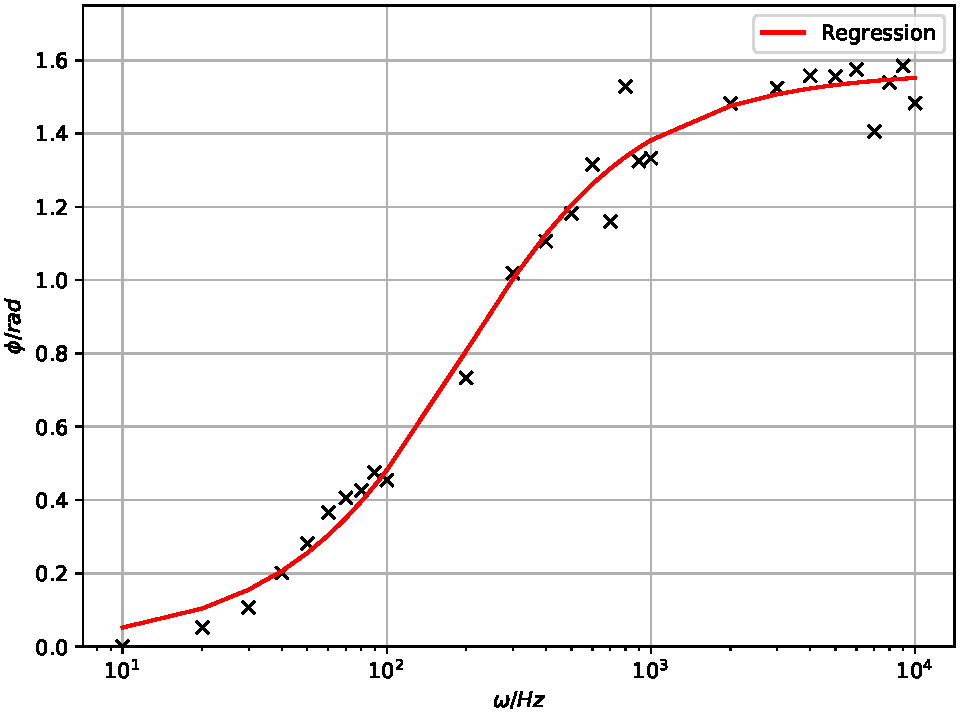
\includegraphics[width=\textwidth]{Diagramm3.pdf}
  \caption{Diagrammdarstellung von der Phasenverschiebung in Abhängigkeit von der Frequenz}
  \label{fig:8}
\end{figure}
Dabei wird die Gleichung (\ref{eq:6}) verwendet und umgeschrieben:
\begin{equation*}
  \phi= arctan(m*\omega)
\end{equation*}
\centerline{Dabei ist $m=(5,228 \pm \, 0,259) \cdot 10^{-3} \si{\second}$} \\
Wie auch hier ist $m$ die Zeitkonstante $RC$.\\
Nun wird die relative Amplitude in Abhängigkeit der Phase in einen Polarkoordinaten aufgetragen.
\begin{figure}[H]
  \centering
  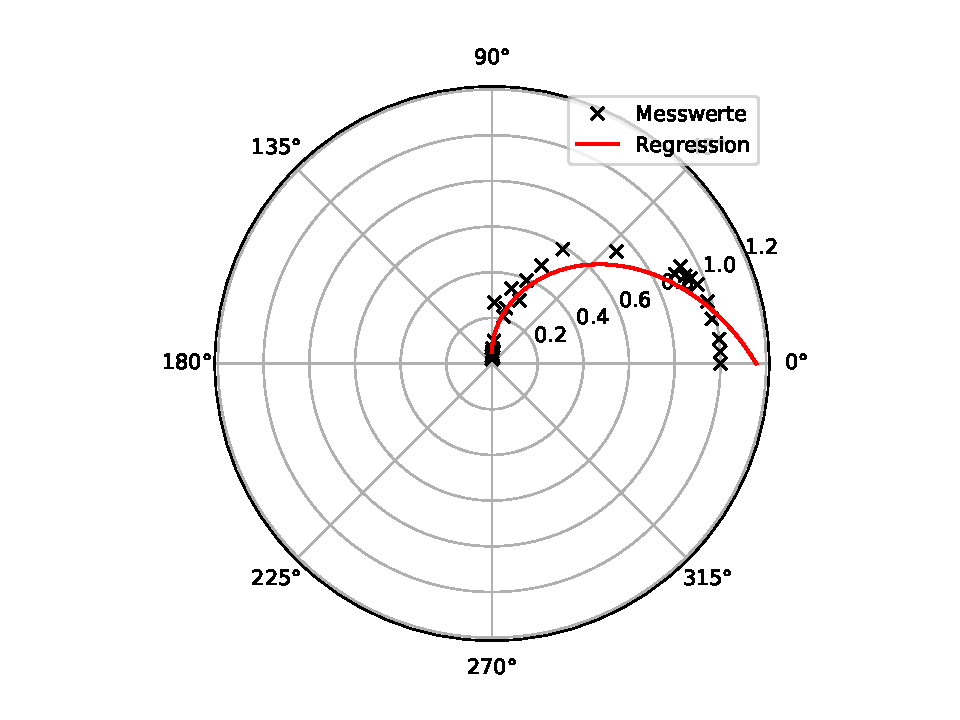
\includegraphics[width=\textwidth]{Polar.pdf}
  \caption{Polarkoordinatendarstellung}
  \label{fig:9}
\end{figure}
\subsection{Integrator}
In diesem Fall wird die Gleichung (\ref{eq:8}) verwendet. \\
\centerline{1.Fall Sinusspannung}
\begin{equation*}
  f(x) = A * sin(x) \rightarrow F(x)= - A * cos(x)
\end{equation*}
\begin{figure}[H]
  \centering
  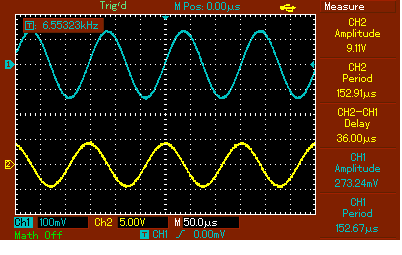
\includegraphics[width=\textwidth]{sinus.png}
  \caption{Thermodruck von der Sinusspannung}
  \label{fig:10}
\end{figure}
Auf dem Thermodruck zeigt, dass die Integration über die Funktion f(x) die
Stammfunktion F(x) ergibt.\\
\centerline{2. Fall Dreieckspannung}
\begin{align*}
  f_1 (x) = c \cdot x \, \text{für} \, -a \leq x \leq a \\
  f_2 (x) =-c \cdot x \, \text{für} \, a \leq x \leq 3a \\
\end{align*}
Die Integrationen für diese Funktion f(x) lauten:
\begin{align*}
  F_1 (x) = \frac{c}{2} \cdot x^{2} \, \text{für} \,-a \leq x \leq a \\
  F_2 (x) = -\frac{c}{2} \cdot x^{2} \, \text{für} \, a \leq x \leq 3a \\
\end{align*}
\begin{figure}[H]
  \centering
  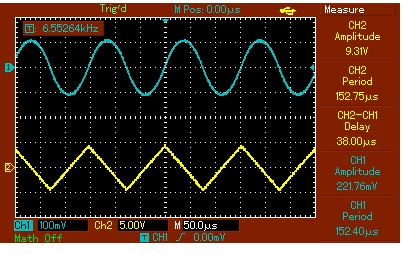
\includegraphics[width=\textwidth]{Dr1.png}
  \caption{Thermodruck von der Dreieckspannung}
  \label{fig:11}
\end{figure}
Der Thermodruck zeigt auch hier das die Funktion f(x) die Stammfunktion F(x) ergibt.\\\\
\centerline{3.Fall Rechteckspannung}
\begin{align*}
f_1 (x) =  c \,\, \text{für} \,\, 0 \leq x \leq a \\
f_2 (x) =  -c \,\, \text{für} \,\, a\leq x \leq 2a
\end{align*}
Durch Integration über die Funktion $f_1 (x)$ und $f_2 (x)$ ergibt sich:
\begin{align*}
  F_1 (x) =  c\cdot x \, \text{für} \, 0 \leq x \leq a \\
  F_2 (x) =  -c\cdot x \, \text{für} \, a\leq x \leq 2a
\end{align*}
\begin{figure}[H]
  \centering
  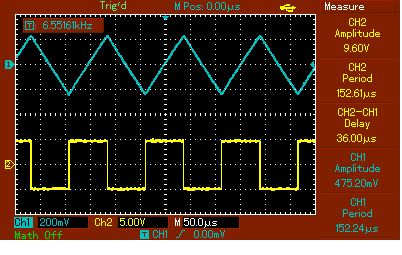
\includegraphics[width=\textwidth]{Re.png}
  \caption{Thermodruck von der Rechteckspannung}
  \label{fig:12}
 \end{figure}
